
The system is divided into `bins' and for each bin $j=1,...M$ we evaluate the number $n_{j,c}$
of particles of species $c=1,...C$.
The joint probability that a particle of species $c$
is in bin $j$ can be calculated by dividing $n_{j,c}$ by the overall system population.

\begin{equation}
p_{j,c} = \frac{\frac{n_{j,c}}{P_c}}{\sum\limits_{i=1}^M \sum\limits_{c=1}^C \frac{n_{i,c}}{P_c}}
\label{eq:shannon1}
\end{equation}
with 
\[
P_c = \frac{n_c}{M}
\]
where $n_c$ is the total number of particles of $c$ in the domain.
Using the joint probabilities of the equation above we then calculate the entropy:
\begin{equation}
S= -\sum_{j=1}^M \sum_{c=1}^C p_{j,c} \ln p_{j,c}
\label{eq:shannon2}
\end{equation}
Note that if one starts with $n_1=n_2=...n_C$ then all values of $P_i$ are equal and 
therefore can be removed from Eq.~\eqref{eq:shannon1} and the denominator is then simply 
the total number of particles in the domain.

Eq.~\eqref{eq:shannon2} can be expressed as the sum of two other entropies:
the conditional entropy $S_{location}(species)$ and the entropy of spatial 
distribution $S(location)$, i.e.:
\[
S=S_{location}(species) + S(location)
\]

We have 
\[
p_{j,c} = p_{c|j}p_j
\qquad
\text{with}
\qquad
p_{c|j}=\frac{\frac{n_{j,c}}{P_c}}{\sum\limits_{c=1}^C \frac{n_{j,c}}{P_c}}
\qquad
\text{and}
\qquad
p_j =\frac{\sum\limits_{c=1}^C \frac{n_{j,c}}{P_c}}{\sum\limits_{i=1}^M \sum\limits_{c=1}^C \frac{n_{i,c}}{P_c}} 
\]
Substituting Eq.~\eqref{} into Eq.~\eqref{}:
\begin{eqnarray}
S
&=& -\sum_{j=1}^M \sum_{c=1}^C p_{j,c} \ln p_{j,c} \nn\\
&=& -\sum_{j=1}^M \sum_{c=1}^C \left[ (p_{c|j}p_j) \ln (p_{c|j}p_j) \right] \nn\\
&=& -\sum_{j=1}^M \sum_{c=1}^C \left[ (p_{c|j}p_j) \ln (p_j) \right] 
    -\sum_{j=1}^M \sum_{c=1}^C \left[ (p_{c|j}p_j) \ln (p_{c|j}) \right] \nn\\
\end{eqnarray}
Since $\sum\limits_{c=1}^C p_{c|j}=1$, then:
\begin{eqnarray}
S
&=&-\sum_{j=1}^M \left[
p_j \sum_{c=1}^C p_{c|j} \ln p_{c|j}
\right]
-
\sum_{j=1}^M p_j \ln p_j \nn\\
&=& 
\underbrace{S_{location}(species)}_{S_2} + \underbrace{S(location)}_{S_3}
\end{eqnarray}



--------------------------------------------------------------


As specified in the paper we also use a 4th order Runge-Kutta (in space only here)
with a fixed timestep $\delta t=10^{-6}$.
We then expect 3 stagnation points at $(0.5,0.5)$ and $(0.5,0.5\pm 0.161)$.

This \stone borrows from \stone~76 (Q2P-1 element), \stone~13 for PIC, \stone~67 for Runge-Kutta algorithms.

%--------------------------------------------------------------------

\begin{center}
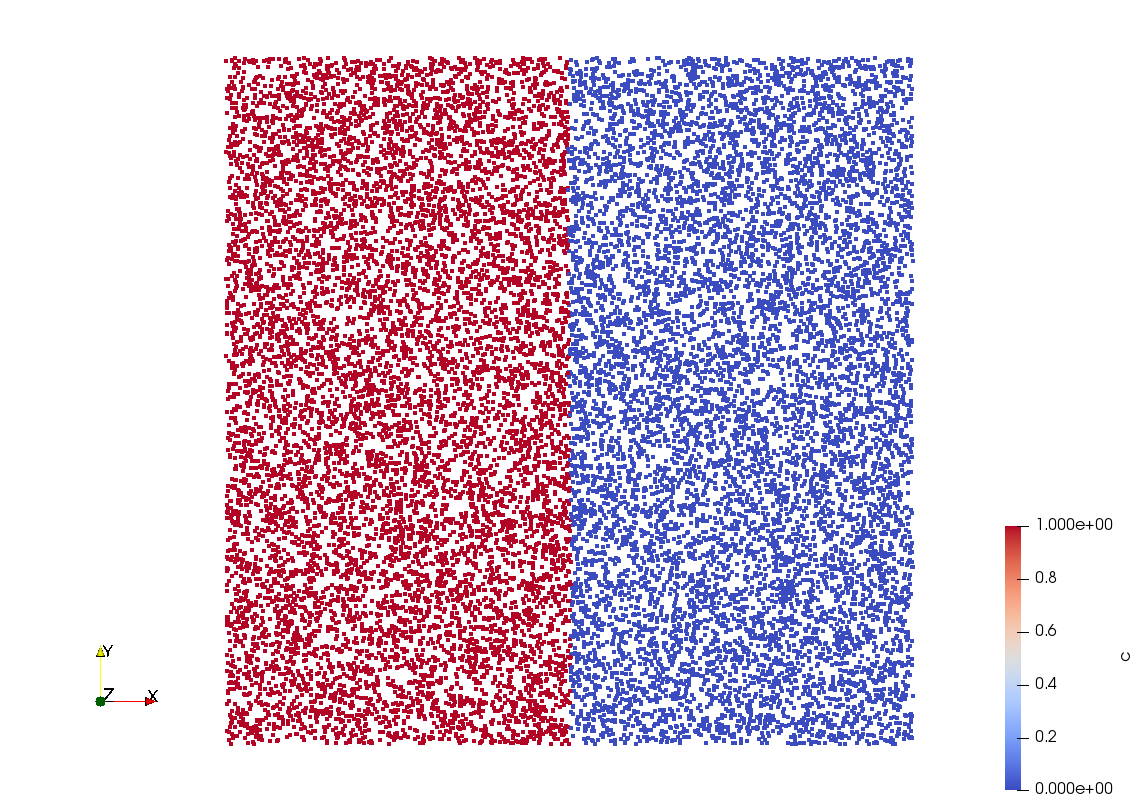
\includegraphics[width=4cm]{python_codes/fieldstone_137/images/exp_1}
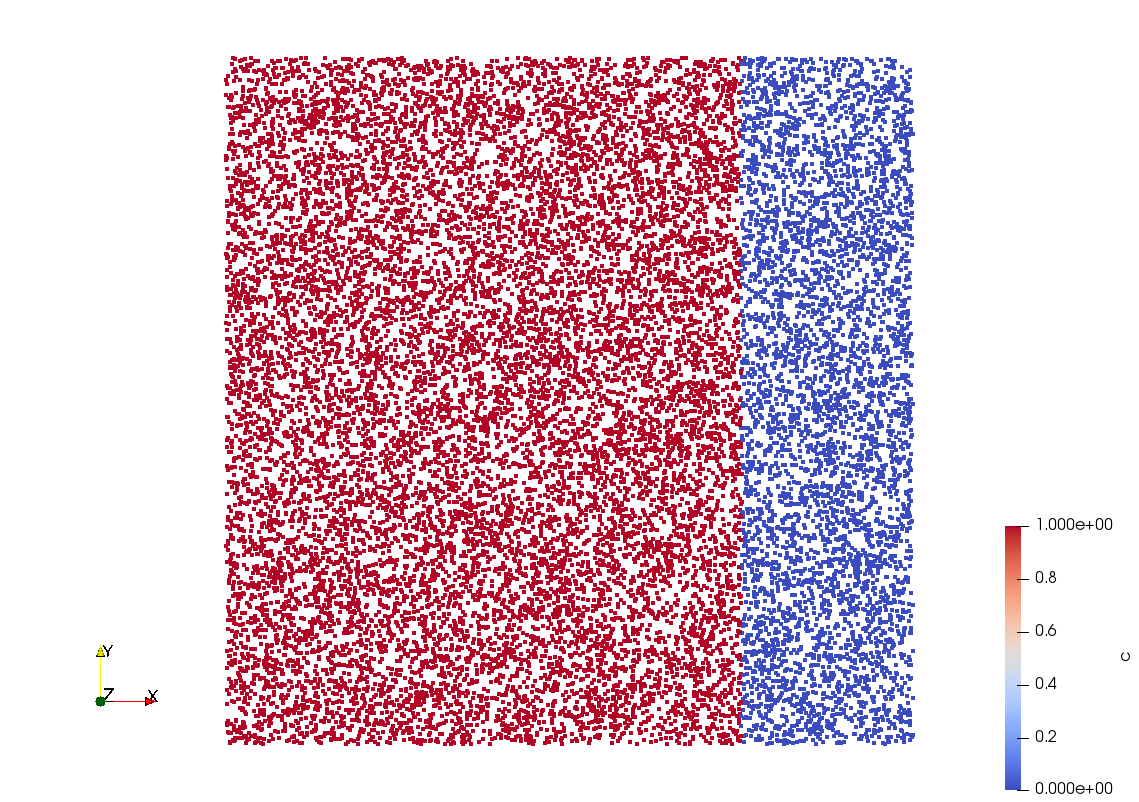
\includegraphics[width=4cm]{python_codes/fieldstone_137/images/exp_2}
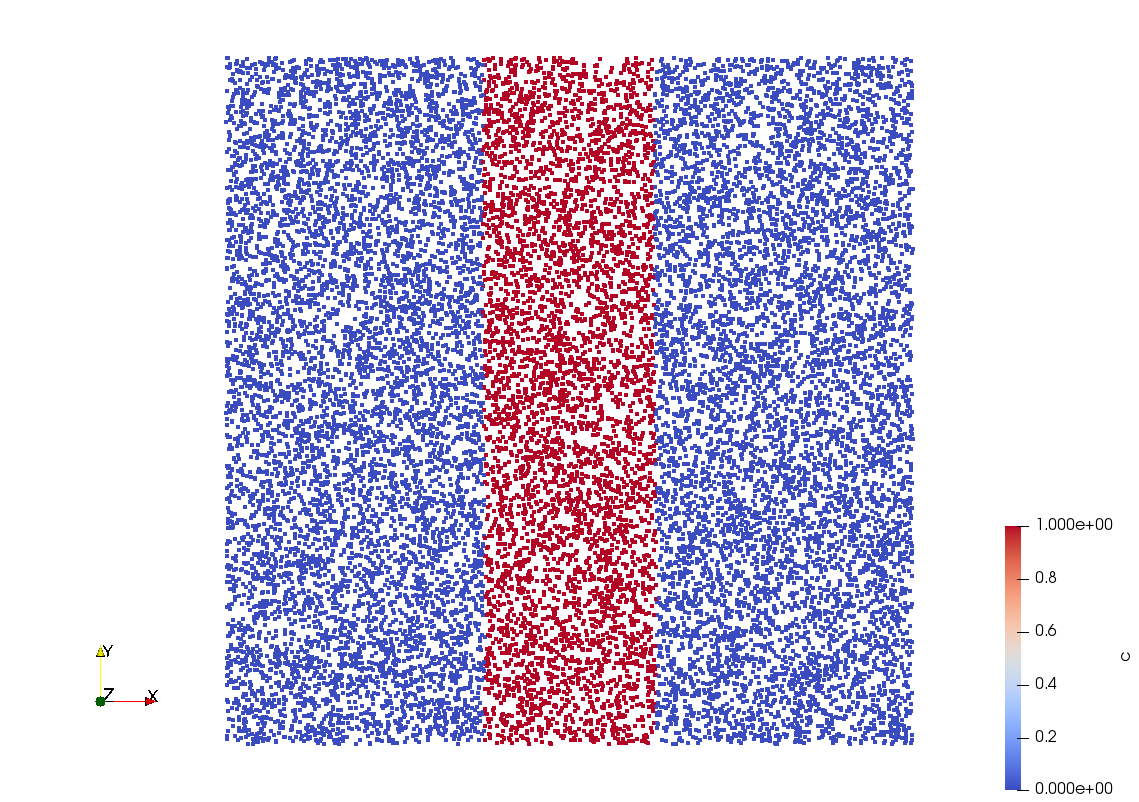
\includegraphics[width=4cm]{python_codes/fieldstone_137/images/exp_3}
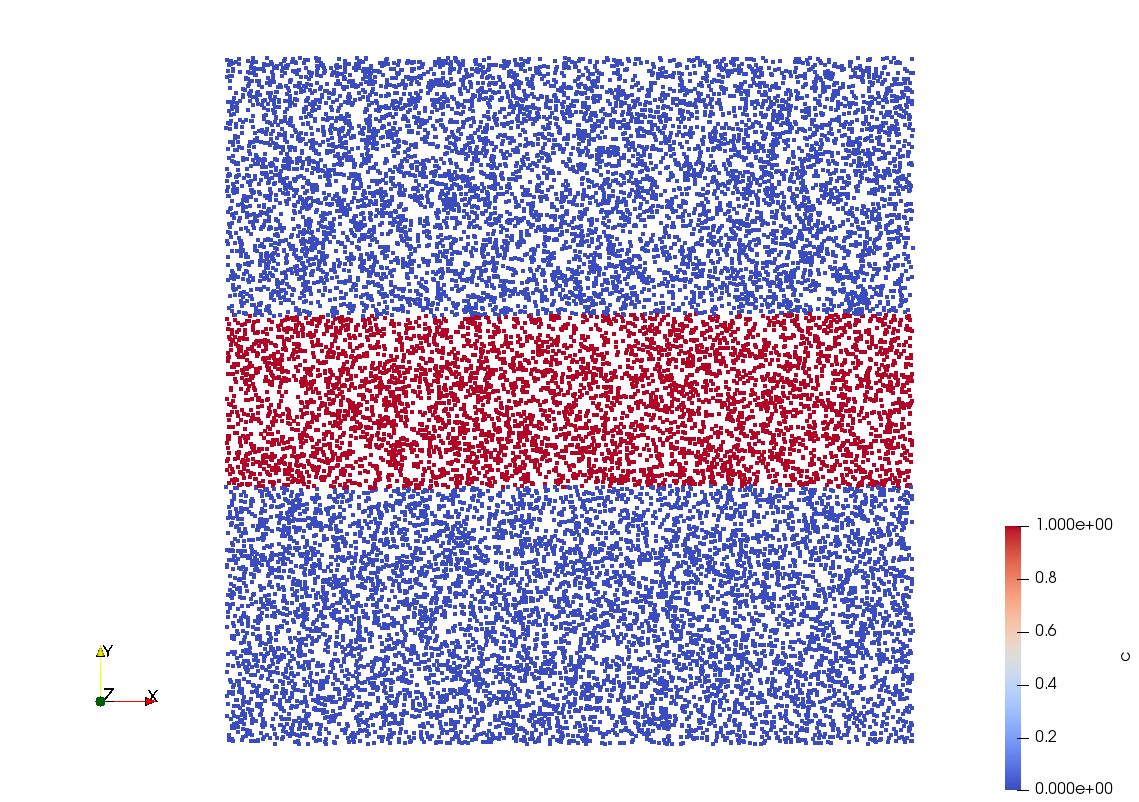
\includegraphics[width=4cm]{python_codes/fieldstone_137/images/exp_4}\\
{\captionfont From left to right: exp=1,2,3,4.}
\end{center}



%--------------------------------------------------------------------
\subsubsection*{Testing: Using the Donea \& Huerta manufactured solution}

This benchmark is taken from Donea \& Huerta (2003) \cite{dohu03} and is described fully 
in section \ref{mms1}. 
We here explore the influence on $S$ of the Runge-Kutta order, the value of the CFL number and 
the mesh resolution for a given number of 10x10 bins. 

\begin{center}
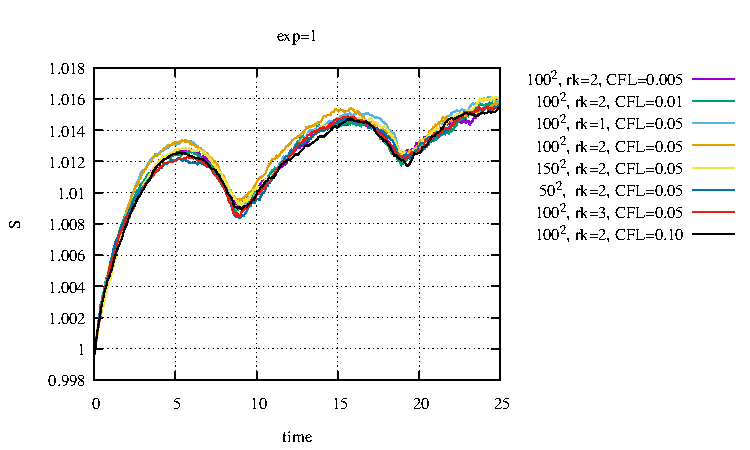
\includegraphics[width=7cm]{python_codes/fieldstone_137/exp1/S.pdf}
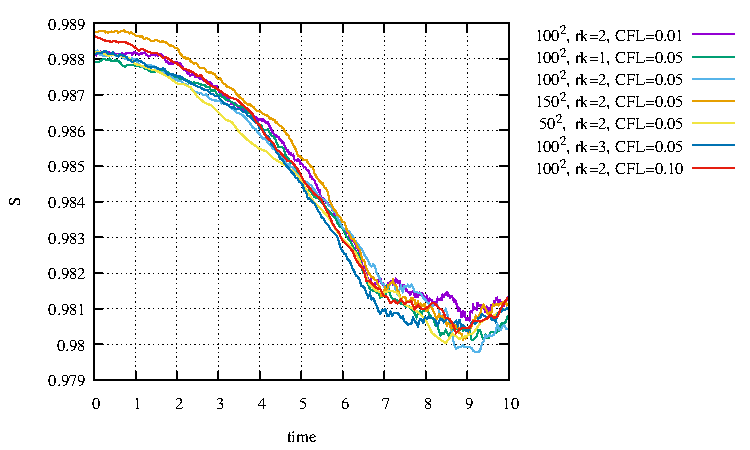
\includegraphics[width=7cm]{python_codes/fieldstone_137/exp2/S.pdf}\\
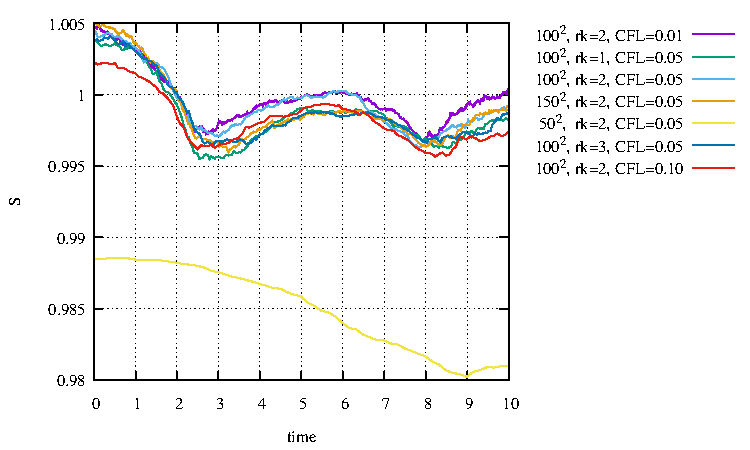
\includegraphics[width=7cm]{python_codes/fieldstone_137/exp3/S.pdf}
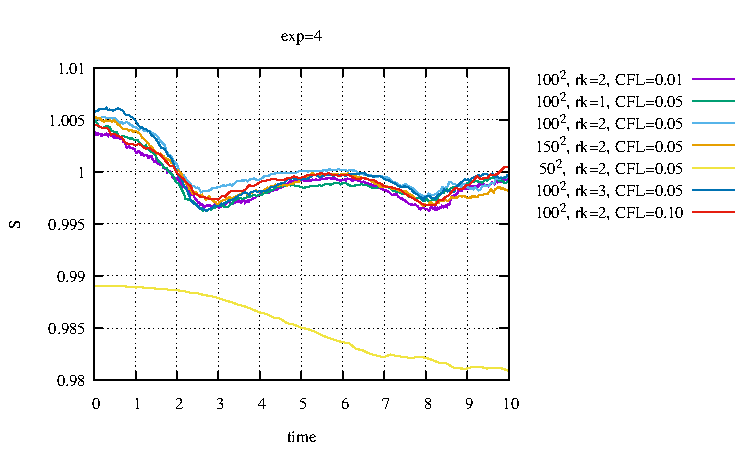
\includegraphics[width=7cm]{python_codes/fieldstone_137/exp4/S.pdf}\\
{\captionfont Left: exp1, right: exp2. $S$ normalised by $\ln{M}$.}
\end{center}

Q: why is S equal to log(M) ?


%--------------------------------------------------------------------
\subsubsection*{Reproducing results of \textcite{cakm06}?}

The domain is a unit square. Boundary conditions are no slip on the sides, 
$\vec\upnu=(1,0)$ at the top and $\vec\upnu=(-1,0)$ at the bottom.
The flow is assumed to be isoviscous ($\eta=1$), incompressible and isothermal. 
Gravity is set to zero.
Note that the original paper \cite{cakm06} solves the Navier-Stokes equations but with $Re=1$
so as to avoid turbulence.
Also the authors state that ``the velocity is not a function of time'' which I interprete as 
them solving the steady state N-S equations. 

